\documentclass{article} 
\usepackage{tikz}
\usepackage{darkmode}
\enabledarkmode
\usepackage[a4paper]{geometry}
\usepackage{fancyhdr}
\pagestyle{fancy}
\lhead{Ökologie}
\rhead{Februar 2025}
\begin{document}
 
\section*{Kurzfassung}
Die wichtigsten Begriffe auf einen Blick \newline
\begin{center}
\begin{tabular}{ |c|c| }
\hline
 \multicolumn{2}{|c|}{\textbf{Ökosystem}} \\
\hline
 \textbf{Biotop} & \textbf{Biozönose} \\
\hline
 nicht lebendig & lebendig, biologisch \\
\hline
 \textbf{a}biotische Umweltfaktoren & biotische Umweltfaktoren \\
\hline
\end{tabular}
\end{center} 
 
\begin{center}
\begin{tabular}{ |c|c| } 
\hline
 \multicolumn{2}{|c|}{\textbf{Potenzen}} \\ 
\hline
 \textbf{physiologisch} & \textbf{ökologisch} \\
\hline
 experimentell & realitätsnah \\
\hline
 optimale Lebensbedingung & weitere Umweltfaktoren \\
\hline
 keine Konkurrenz & Konkurrenz \\
\hline
\end{tabular}
\end{center}
 
\begin{center}
\begin{tabular}{ |c|c| } 
\hline
 \multicolumn{2}{|c|}{\textbf{Toleranzkurven}} \\ 
\hline
 \textbf{Begriff} & \textbf{Erklärung} \\
\hline
 \textbf{Toleranzkurven} & Kurve der Potenz nach einem Umweltfaktor \\
\hline
 \textbf{Minimum / Maxiumum} & Minimale / Maximale belebbares vorkommen der Umweltfaktors \\
\hline
 \textbf{Optimum} & Punkt der höchsten Potenz \\
\hline
 \textbf{Präferenzbereich} & Bereich um das Optimum \\
\hline
 \textbf{Pessimum} & Bereich um enden, belebbar, nicht fortpflanzbar \\
\hline
\end{tabular}
\end{center}  
Eine 2D Toleranzkurve ist ein Ökogramm.   
 
\begin{center}
\begin{tabular}{ |c|c| } 
\hline
 \multicolumn{2}{|c|}{\textbf{Regeln}} \\ 
\hline
 \textbf{Bergmannsche Regel} & Je kälter die Klimazone, desto größer das Tier \\
\hline
 \textbf{Allensche Regel} & Je wärme die Klimazone, desto größer die Körperanhänge \\
\hline
\end{tabular}
\end{center}
 
 
\section{Ökosystem}  
\begin{description} 
\item[dynamisch] Ökosysteme konenn durch Einflüsse, den \textbf{Umweltfaktoren}, sowohl von Innen und Außen verändert werden. 
\item[komplex] Die einzelnen Bestandteile eines Ökosystems wirken in einem komplexen Geflecht dauerhaft unterschiedlich aufeinander ein.
\item[offen] Es gibt keine klar definierten Grenzen zwischen mehreren Ökosystemen, sie gehen ineinander über. Lebewesen (und auch Energie) können sich frei zwischen mehrere Ökosystemen bewegen.
\end{description} 
 
\noindent Ein Ökosystem setzt sich aus der \textbf{Biozönose}, allen dort lebenden Lebewesen, und dem \textbf{Biotop}, dem nicht lebendigem Lebensraum der Lebewesen. Bäume o.ä. sind auch Lebewesen. \newline
Umweltfaktoren durch das Biotop, wie das Grundwasser, der Boden oder der Niederschalg, sind \textbf{abiotisch}. Umweltfaktoren der Biozönose, wie Zellatmung und Fotosynthese oder Konkurrenz zwischen Organismen, sind \textbf{biotisch}. Abiotische und biotische Umweltfaktoren können auch auf den jeweils anderen Teil des Ökosystems einwirken: abiotische Faktoren wirken sich viel auf die Biozönose aus und biotische Faktoren können sich auch auf das Biotop auswirken.
 
\section{Potenz} 
Die Potenz gibt an, in welchem Bereich eines Umweltfaktores ein Lebewesen überleben und sich fortpflanzen kann. Dabei wird unterschieden in \textbf{physiologische} und \textbf{ökologische} Potenzen, jeweils in laborisch experimentell hergestellten Optimalbedingungen und unter realitätsnahen Einflüssen von durch andere Umweltfaktoren. \newline
Diese können komplett verschieden sein, wie z.B. bei den Trespen der Hohenheimer Grundwasserversuch, welche eine sehr breite physiologische Potenz haben und auch in trockenen Regionen wachsen könnten, dort aber von anderen Pflanzen konkurrenz geboten werden, weshalb es nicht teil der ökologischen Potenz ist.
 
\subsection{Toleranzkurve}
Die Toleranzkurve ist eine kurve, der Normalverteilung ähnlich, welche die Potenz eines Lebewesens basierend auf einen Umweltfaktor darstellt. Die gesamte Kurve zeigt den \textbf{Toleranzbereich}, den Bereich, in dem Lebewesen leben können. An den enden ist das \textbf{Minimum und Maximum}. In der Mitte ist das \textbf{Optimum}, der Bereich um das Optimum ist der \textbf{Präferenzbereich}. Kurz vor den enden bis zu den enden, die zwei Bereiche mit der geringsten Potenz, können Lebewesen gradeso überleben aber sich nicht fortpflanzen. Das ist das \textbf{Pessimum}.
  
\begin{figure}[h] 
  \centering
  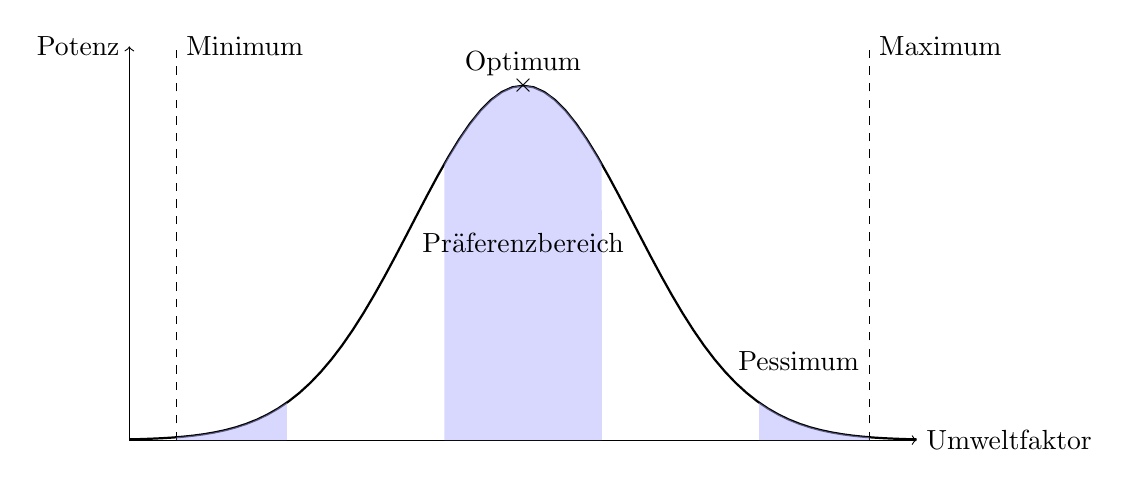
\begin{tikzpicture}     
    \draw[thick, domain=-5:5, samples=75] 
            plot (\x, {4.5*exp(-0.5*\x*\x*0.5)});
     
    \draw[->] (-5,0) -- (5,0) node[right] {Umweltfaktor};
    \draw[->] (-5,0) -- (-5,5) node[left] {Potenz}; 
    
    \draw[dashed] (-4.4,0) -- (-4.4, 5) node[right] {Minimum};    
    \draw[dashed] (4.4,0) -- (4.4, 5) node[right] {Maximum};
 
    \fill[blue!30, opacity=0.5] (-1,0) -- plot[domain=-1:1, smooth, samples=10] (\x, {4.5*exp(-0.5*\x*\x*0.5)}) -- (1,0) -- cycle;
  
    \draw[] (0,4.5) node {$\times$} node[above] {Optimum};
    \node[] at (0,2.5) {Präferenzbereich};
 
    \fill[blue!30, opacity=0.5] (-4.4,0) -- plot[domain=-4.4:-3, smooth, samples=10] (\x, {4.5*exp(-0.5*\x*\x*0.5)}) -- (-3,0) -- cycle;  
    \fill[blue!30, opacity=0.5] (3,0) -- plot[domain=3:4.4, smooth, samples=10] (\x, {4.5*exp(-0.5*\x*\x*0.5)}) -- (4.4,0) -- cycle;
 
    \node[] at (3.5, 1) {Pessimum};
  \end{tikzpicture}
\end{figure} 
 
\subsection{Ökogramm}
Ein Ökogramm ist unterm Strich eine zweidimensionale Toleranzkurve, welche die Potenz nach zwei Umweltfaktoren zeigt.
 
\subsection{Die Bergmannsche Regel}
Die Bergmannsche Regel besagt, dass nah verwandte Tierarten in der Regel in kälteren Klimazonen größer sind. Dies liegt daran, dass das energieproduzierende und speichernde Volumen als kubische Funktion schneller anwächst als die wärmeabgebende Oberflächen. Größere Tiere geben zwar etwas mehr Wärmeenergie als kleinere Tiere ab, können aber auch um ein Vielfaches mehr Wärmeenergie produzieren und speichern, welches für das Überleben in kalten Regionen lebensnotwendig ist.
 
\subsubsection{Ausnahmen}
Tiere wie beispielsweise der sehr Adelie-Pinguine können auch in kalten Regionen überleben, obwohl sie klein sind, weil sie stattdessen auf andere Art und Weise sich wärmen, wie durch proteinreiche Ernährung und eine erhöhte Körperaktivität.
 
\subsection{Die Allensche Regel}
Je wärmer die Klimazone ist, in der ein nah verwandtes Tier lebt, desto größer sind dessen Körperanhänge wie Ohren. Dadurch dass die größer sind haben sie eine größere Oberfläche und können besser Wärmeenergie abgeben und somit die Temperatur des Tiers regulieren.
\end{document}
 
 
 
 
